%! TEX root = ../thesis.tex

\chapter{Extensive air showers}
\label{chapter:extensive-air-showers}

Consider a high energy cosmic ray impinging on earth. The questions pertaining to where it might originate from and how it has gained so much kinetic energy have 
been answered in the preceding \autoref{chap:physical-background}. In the following, the particle cascades resulting from the particle interacting in the upper
atmosphere will be examined. This is done in a two-fold way. The underlaying principles will be explained via considering a particle carrying no SU$(3)$-color 
charge in \autoref{sec:heitler-model}. The more general treatment for hadronic showers is then found in \autoref{sec:heitler-matthews-model}. As supplementary 
information, the effect of different hadronic primaries is discussed in \autoref{sec:superposition-principle}.

\section{Electromagnetic showers}
\label{sec:heitler-model}

\begin{figure}
	\begin{subfigure}[b]{0.4\textwidth}
		\centering
		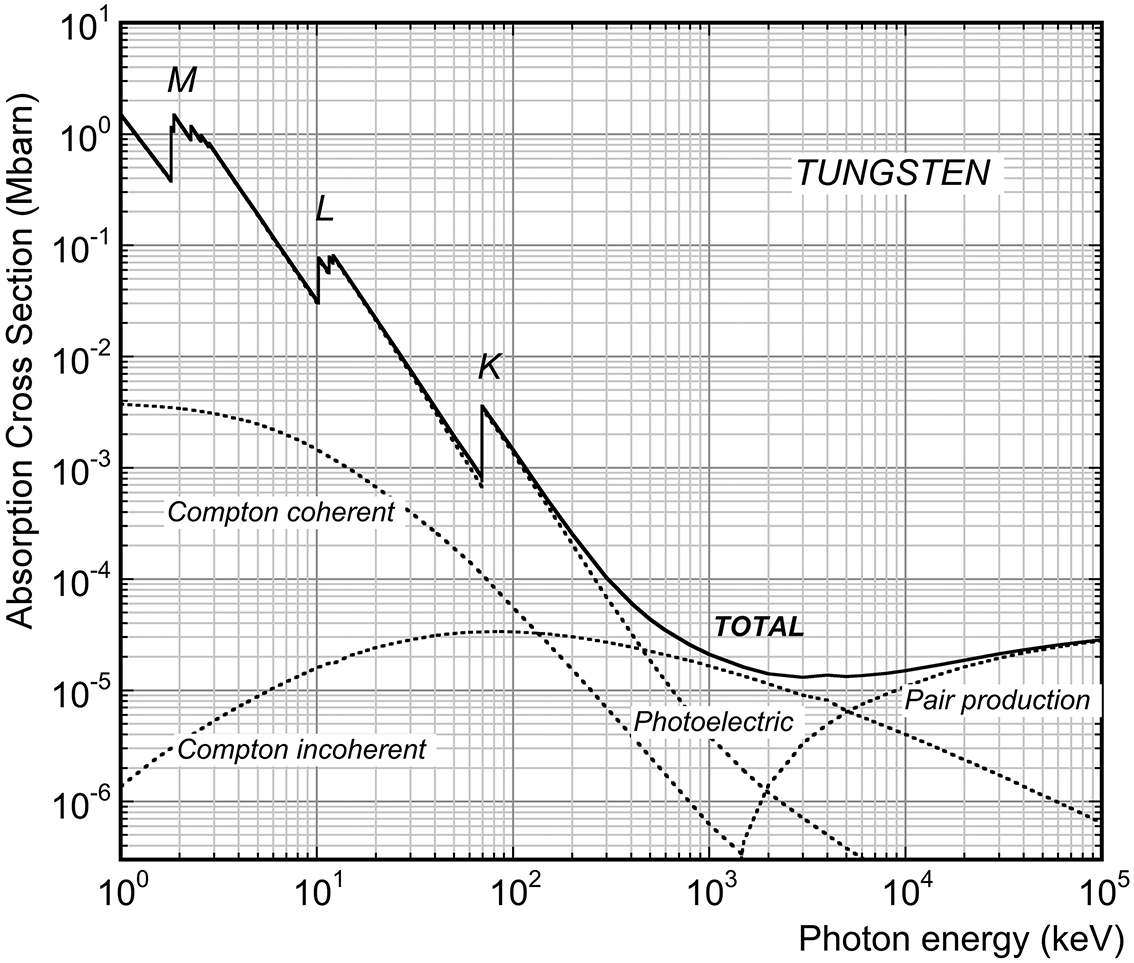
\includegraphics[width=\textwidth]{./plots/photon_cross_section.png}
		\caption{$\mathbf{\gamma}$\textbf{ interactions}}
		\label{fig:gamma-interactions}
	\end{subfigure}
	\hfill
	\begin{subfigure}[b]{0.6\textwidth}
		\centering
		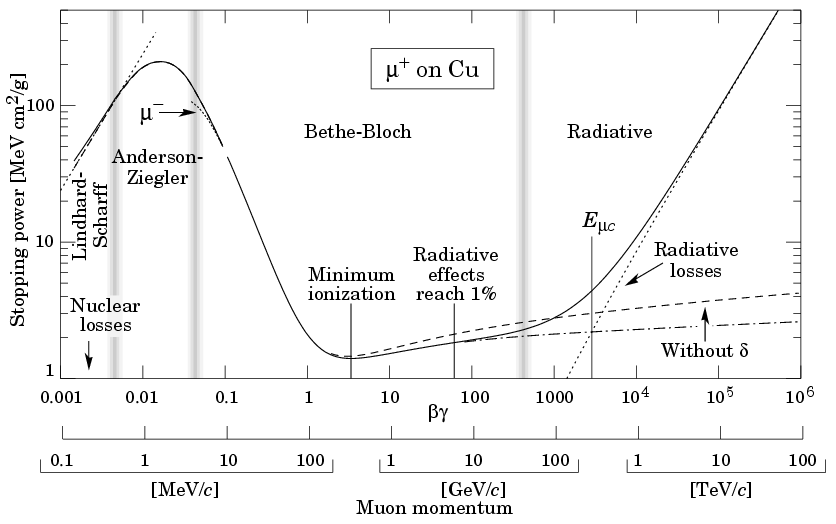
\includegraphics[width=\textwidth]{./plots/electron_ionisation_loss.png}
		\caption{$\mathbf{e^\pm}$\textbf{ interactions}}
		\label{fig:electron-interactions}
	\end{subfigure}
	\caption{\textbf{(a)} Cross section for different energy loss processes of a photon in tungsten. The sudden spikes correspond to the transition energy of 
	increasingly higher-energy electron shells. From \cite{chen2007interactions}. \textbf{(b)} Stopping power of copper, representatively on an antimuon $\upmu^+$, 
	with respect to its' momentum. Plot adopted with changes from \cite{meroli2017straggling}.}
	\label{fig:ionization-losses}
\end{figure}

The dominating interaction of $E > \SI{10}{\mega\electronvolt}$ photons in matter is $e^+e^-$ pair production, whereas for electrons/positrons the creation of a
$\gamma$ via bremsstrahlung prevails at high energies. This is shown in \autoref{fig:ionization-losses}. Consequently, an entire cascade of electrons, positrons 
and photons can emerge from a single primary particle, as realised by Heitler in \cite{heitler1984quantum}. 

Of particular interest in these showers are, apart from the primary particles energy $E_0$ and arrival direction $(\Upphi, \theta)$, the atmospheric depth 
$X_\text{max}$ at which it reaches its' maximum multiplicity, as well as the \textbf{L}ateral \textbf{D}istribution \textbf{F}unction (LDF), that parametrizes the 
distribution of particles along the shower axis. An important variable that influences both values is the radiation length $X_0$. It represents the characteristic
length at which an $e^\pm$ loses $1-\frac{1}{e}\approx63\%$ of its energy. It also corresponds to the mean free path of a photon in matter up to a factor $7 / 9$ 
\cite{gupta2010calculation}. Neglecting said factor and assuming that new particles on average inherit half of the original energy, describing the multitude of 
particles contained in an electromagnetic shower becomes a counting exercise in the context of the Heitler-model.

With each radiation length, the number of particles $N$ in the shower double, while the energy per particle $E_\text{pp}$ halves. After traversing an atmospheric 
depth of $n\cdot X_\text{max}$, typically measured in \SI{}{\gram\per\centi\meter\squared}, they consequently read

\begin{equation}
\label{eq:heitler-parameters}
N(n) = 2^n, \qquad E(n) = \frac{E_0}{2^n}.
\end{equation}

After some time, the energy of each individual particle $E_\text{PP}$ will have diminished by so much that other processes will dominate over bremsstrahlung and 
pair production. This occurs at the critical energy $E_c$ below which the shower rapidly stops creating new particles and dies out as a result. It follows via 
\autoref{eq:x-max} and \ref{eq:n-max} that both $X_\text{max}$ as well as $N_\text{max}$ increase with $E_0$. The multiplicity arising from 
these assumptions alongside a stylized propagation of the thus created shower is represented in \autoref{fig:heitler-model}. 

\begin{align*}
E_\text{PP}\,(n_\text{max}) &\stackrel{!}{=} E_c \stackrel{\eqref{eq:heitler-parameters}}{=} \frac{E_0}{2^{n_\text{max}}}\\
\Leftrightarrow \qquad \qquad n_\text{max} &= \left\lfloor \log_2 \left( \frac{E_0}{E_c} \right) \right\rfloor \\[7pt]
\Rightarrow \qquad \qquad\!\! X_\text{max} &= n_\text{max}\cdot X_0 = \left\lfloor \log_2 \left( \frac{E_0}{E_c} \right) \right\rfloor. \numberthis\label{eq:x-max} \\
\Rightarrow \qquad \qquad\!\! N_\text{max} &= 2^{n_\text{max}} = \left\lfloor \frac{E_0}{E_c} \right\rfloor. \numberthis\label{eq:n-max}
\end{align*}

\begin{figure}
	\centering
	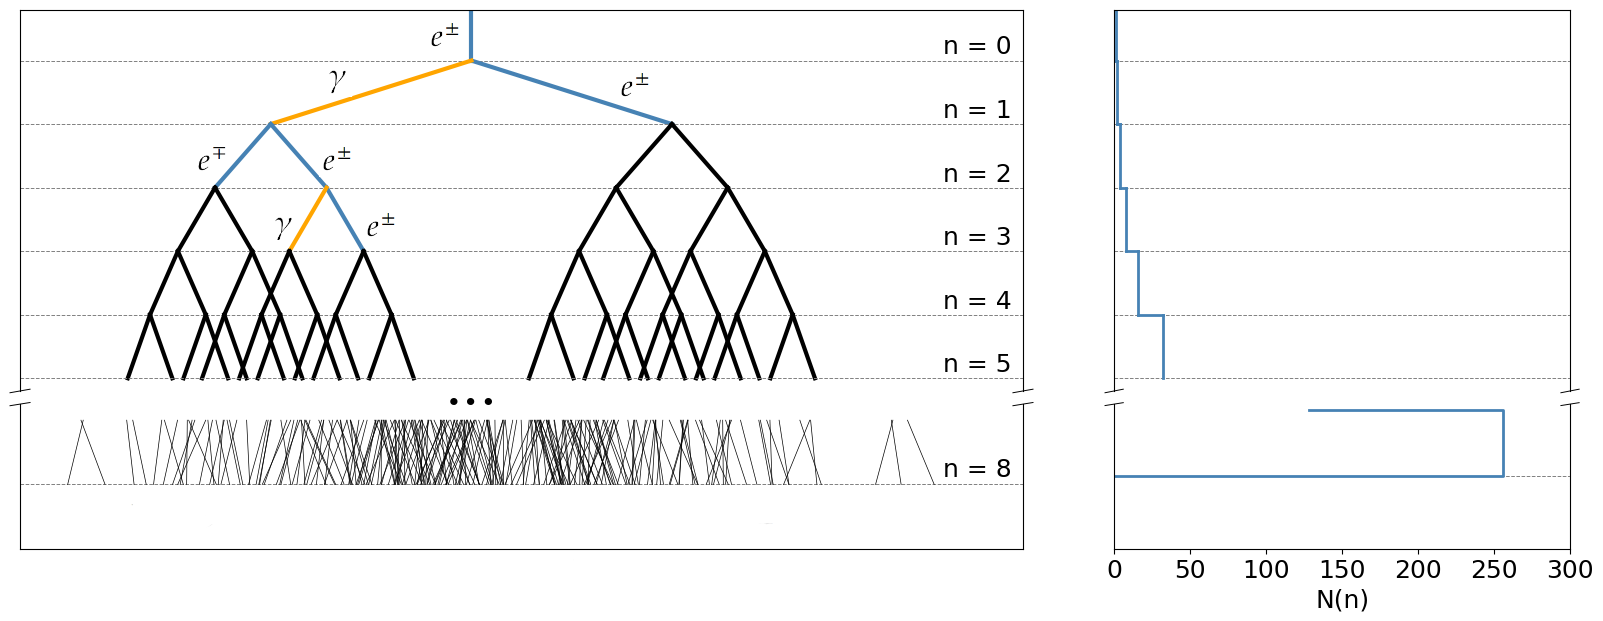
\includegraphics[width=\textwidth]{./imgs/heitler_shower.png}
	\caption{Shown on the left is the stylized propagation of an extensive air shower through the atmosphere according to the Heitler-model, quantized in units
	of $X_0$. The energy of the primary particle is of order $2^8\cdot E_c$, which allows for 8 bifurcation steps, and $N_\text{max}=256$ shower particles. The
	multiplicity of the shower after each step is shown in the right subplot.}
	\label{fig:heitler-model}
\end{figure}

The number of particles at a given distance from the shower axis (y-axis in \autoref{fig:heitler-model}) is essentially random, but follows a statistical basis,
the lateral distribution function. The LDF can either be derived approximately from first principles \cite{kamata1958lateral} or empirically, as is done in 
\cite{greisen1960cosmic}. The latter arrives at a closed form approximation for the local density $\rho$ of particles given a shower with multiplicity $N$ at a 
distance $r$ from the shower axis as

\begin{equation}
\label{eq:NKG-electrons}
\rho_\text{EM}(N, r)=\frac{0.4\,N}{r_\text{M}^2} \left(\frac{r_\text{M}}{r}\right)^{0.75} \left(\frac{r_\text{M}}{r+r_\text{M}}\right)^{3.25}\left(1+\frac{r}{11.4\,r_\text{M}} \right).
\end{equation}

In \autoref{eq:NKG-electrons}, the Molière radius $r_\text{M}$ characterizes the lateral spread in multiple scattering processes. It is of order 
$r_\text{M}\approx\SI{100}{\meter}$ for interactions that are relevant here, and in general depends on the density of the considered material 
\cite{moliere1947theorie}.

\section{Hadronic showers}
\label{sec:heitler-matthews-model}

Hadronic primaries will readly produce color-charged secondaries, as has been shown many times in particle accelerators. In order to model the development of 
hadronic showers, the model discussed in \autoref{eq:heitler-parameters} thus needs to be adjusted. An example theory has been developed by Matthews in 2005. 
Following the reasoning in \cite{matthews2005heitler}, after traversing an atmospheric depth corresponding to the hadronic interaction length, a proton creates on 
average $N_\pi \approx 15$ pions, of which two thirds are charged, and one third is uncharged. Each newly created (charged) particle then repeats this process, 
kicking off the shower cascade. The corresponding decay channels of the light $\pi$-mesons with the largest \textbf{B}ranching \textbf{R}atios (BR) are 

\begin{align*}
	\pi^{+} &\rightarrow \upmu^{+} + \nu_\upmu \!\!\!  \qquad\qquad (\text{BR}\approx0.9999,\,\tau=\SI{2.6033e-8}{\second} \; \text{\cite{PDG}}), \\
	\pi^{-} &\rightarrow \upmu + \bar{\nu}_\upmu \qquad\qquad (\text{BR}\approx0.9999,\,\tau=\SI{2.6033e-8}{\second} \; \text{\cite{PDG}}), \\
	\pi^0 &\rightarrow 2\gamma \!\! \qquad\qquad\qquad (\text{BR}\approx0.9882,\,\tau=\SI{8.5e-17}{\second}\; \text{\cite{PDG}}).
\end{align*}

With a mean lifetime of just attoseconds, the $\pi^0$ decay instantly before being able to continue the cascade process. In this fashion, the uncharged particles 
initiate a Heitler shower as discussed in \autoref{sec:heitler-model}, by providing high-energy photons. It follows that every hadronic shower has an electromagnetic 
component. Moreover, assuming that the inherited energy from the parent particle is roughly uniformly distributed among its' children, one third of the remaining
energy in the hadronic component is lost to the electromagnetic component per hadronic interaction length. 

Similar to the reasoning in \autoref{sec:heitler-model}, a primary of given energy initiates a shower of a specific multiplicity $N_\text{max}$. This is reached 
after $n_\text{max}$ steps, where the energy per particle $E_\text{PP}(n_\text{max})$ is below the critical energy $E_c$ at which the mesons ionize rather than 
continue the cascade. After this last step, the charged pions eventually decay into muons and neutrinos. The shower characteristics in the scope of the 
Heitler-Matthews model that describe hadronic showers are thus given by

\begin{equation}
N_\text{had}(n) = \left(\frac{2\,N_\pi}{3}\right)^n,\qquad E_\text{PP}(n) = \frac{E_0}{N_\pi^n},\qquad n_\text{max}=\left\lfloor\log_N\left(\frac{E_0}{E_{c,\,\text{had}}}\right)\right\rfloor,
\end{equation}

wheras the maximum multiplicity (ignoring neutrinos) in the shower is calculated as

\begin{equation}
\label{eq:n-max-matthews}
N_{\text{max},\,1} = \underbrace{ \frac{3}{2}\left( \frac{2}{3}N_\pi\right)^{n_\text{max}}  }_\text{Muon component} + \;\; 
		     \underbrace{\sum\limits_{k = 1}^{n_\text{max}-1} \frac{N(k)}{3} \cdot \left\lfloor 
		     \frac{E_\text{PP}(k) }{E_{c,\,\text{EM}}}\right\rfloor}_\text{EM component}.
\end{equation}

The muons stemming from pion decay follow a different LDF than the electromagnetic component. Again following the analysis in \cite{greisen1960cosmic}, the muonic
LDF can be recovered as

\begin{equation}
\label{eq:NKG-muons}
\rho_\upmu(N, t) = 18\,\left(\frac{N}{10^6 \cdot r}\right)^\frac{3}{4} \cdot \;\,\left(1 + \frac{r}{320}\right)^{-\frac{5}{2}}.
\end{equation}

While the above \autoref{eq:NKG-muons} drops of slower $\mathcal{O}(r^{-\frac{3}{2}})$ compared to the electromagnetic component ($\mathcal{O}(r^{-3})$), the
immediate vicinity of the shower axis contains mostly photons and leptons from the EM subshower. Further out, the muonic component takes over. This is visualized
in \autoref{fig:component-LDF}. Due to this reason, and the fact that muons can carry considerable amounts of energy faraway from the shower axis, the muonic 
footprint of a shower often appears much more "patchy" compared to the EM portion. This knowledge is espically useful when distinguishing between hadron- and 
photon-induced air showers (compare \cite{capistran2015new}).

\begin{figure}
	\centering
	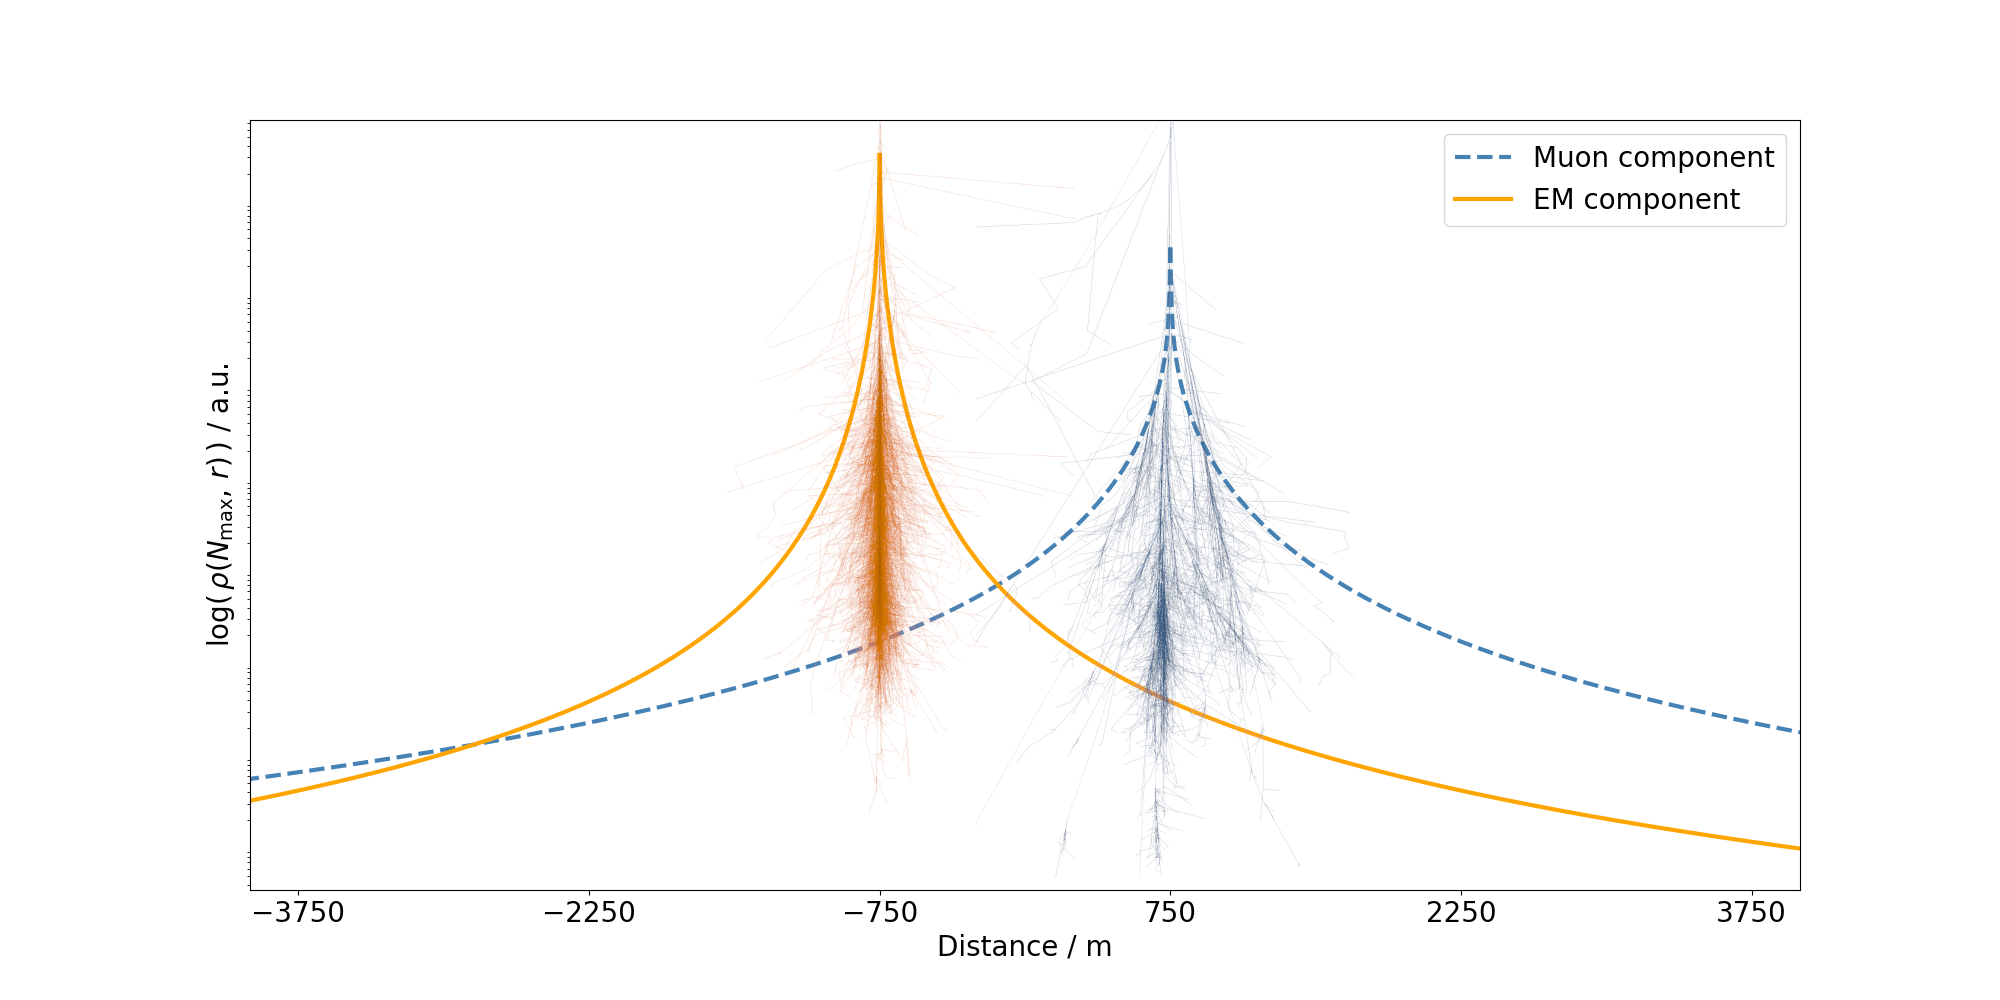
\includegraphics[width=1.0\textwidth]{./plots/componentwise_LDF.png}
	\caption{The lateral distribution function for the muonic (steelblue) and electromagnetic (orange) component of a vertical, \SI{100}{\giga\electronvolt}
	proton shower at roughly sea level ($r_\text{M}=\SI{100}{\meter}$). The inset plots on the top-right represent the xz-projection of the shower shape. Both 
	images adopted with changes from \cite{CorsikaShower}.}
	\label{fig:component-LDF}
\end{figure}

\section{Composite primaries}
\label{sec:superposition-principle}

As is evident from the discussion in \autoref{chap:physical-background}, not only single protons (which are strictly speaking also composite) or elementary 
particles like photons, electrons, etc. appear in the cosmic ray spectrum. Any and all kind of elements can and do appear as possible primaries, given that they
are stable to weak decay and can be effectively accelerated near a CR source. The consequence of different primaries on resulting shower characteristics is subtle,
but large enough such that it can be used for identification purposes.

Assuming the constituents in a CR nucleus all coherently interact with an air molecule, one arrives at the superposition principle for extensive air showers. It 
states that for a composite primary with $A = N + Z$ neutrons and protons, each constituent particle will initiate a shower with initial energy of 
$E_0' = E_0\,/\,A$, where $E_0$ is the initial energy of the composite particle. It follows that air showers from heaver primaries occur at higher altitudes (lower 
atmospheric depth $X$) and with higher particle counts.

\begin{equation}
N_{\text{max},\,A} = A \cdot N_{\text{max},\,1}, \qquad n_{\text{max},\,A} = \left\lfloor \log_N\left(\frac{E_0}{E_{c,\,\text{had}}}\right) - \log_N A \right\rfloor,
\end{equation}

where $N_{\text{max},\,1}$ refers to a proton shower as established in \autoref{eq:n-max-matthews}.

\section{Comments on validity}
\label{sec:cr-shower-validity}

The Heitler model and Heitler-Matthews model discussed in \autoref{sec:heitler-model} and \autoref{sec:heitler-matthews-model} respectively make only very 
rudimentary assumptions on the underlaying physics of particle cascades. Nevertheless, the equations recovered from these assumptions are already a close 
approximation of real world processes up to $X_\text{max}$. 

Of course, adding a stochastic component to the above assumptions (c.f. \cite{MartinShowerSim}) improve predictions, but even full-fledged Monte-Carlo simulation 
software frameworks like GEANT4 \cite{agostinelli2003geant4} or CORSIKA \cite{heck1998corsika} show discrepancies between observed and predicted shower 
development. An example of this is presented in \autoref{fig:model-validity}.



\section{Detection methods}
\label{sec:detecion-methods}
